\documentclass[12pt]{article}
\usepackage{enumerate}
\usepackage{mathematics}

\DeclareMathOperator{\diam}{\mathrm{diam}}

\begin{document}

\section{Math 1A Final (Adiredja)}

\subsection*{1.c}

\begin{mdframed}
  In order to find the maximum, we want the derivative of
\begin{align*}
  f(x) = \int_0^x t^2 - 1 \dt.
\end{align*}
We could integrate it explicitly:
\begin{align*}
  f(x) = \left[\frac{t^3}{3} - t \right]_0^x = \frac{x^3}{3} - x.
\end{align*}
So this is a function telling us the area under the curve for a given $x$. Now
we want the maximum of this function, so we have to differentiate:
\begin{align*}
  \ddx \( \frac{x^3}{3} - x \) = x^2 - 1 = (x+1)(x-1)
\end{align*}
But, ``of course'', this was obvious from FTC.

And that is zero at -1, and 1. But at 1, it's a minimum, not a maximum.
\end{mdframed}

\newpage
\subsection*{3.b}
$\lim_{x\to 2} x^2$ is obviously 4. Prove it.\\

\begin{mdframed}
  We want a procedure that, given a distance $\epsilon$ in the output space,
  shows how to pick a distance $\delta$ in the input space. The $\delta$ must satisfy the following:

  For any $x$ within the radius of $\delta$ in the input space, $x^2$ will be
  within the radius of $\epsilon$ in the output space.

  \textbf{Guess}\\
  First we try to ``guess'' a rule giving a $\delta$ in terms of the $\epsilon$.

  If it is true that $x^2$ is within the radius of $\epsilon$, then that's the
  same as saying
  \begin{align*}
    |x^2 - 4| < \epsilon\\
    x^2 < \epsilon + 4\\
    x < \sqrt{\epsilon + 4}\\
  \end{align*}
  Now, we're trying to make a statement about the size of the window in the
  input space. The distance from the point of interest is $x - 2$, and so we
  know that
  \begin{align*}
    x - 2 < \sqrt{\epsilon + 4} - 2.
  \end{align*}
  So that suggests that the following rule will give a $\delta$ satisfying the
  requirement:

  Choose $\delta = \sqrt{\epsilon + 4} - 2$.

  \textbf{Prove}\\
  We know that $2 \pm \delta$ gets mapped onto the boundary of the output
  window (because we chose $\delta$ to have that property).

  Now, we need to prove that it is true that any $x$ within that input window
  will be mapped into the output window.

  Consider some $x$ in the input window. Where does it get mapped to? Answer:
  $x^2$. Also, we know that $x^2 < (2 + \delta)^2$ (because $2+\delta$ is at
  the outer edge of our input window). And, we've \textit{chosen} a value for
  $\delta$: it's $\sqrt{\epsilon + 4} - 2$. So we can write the following
  inequality:
  \begin{align*}
    x^2 < (2 + \sqrt{\epsilon + 4} - 2)^2
  \end{align*}
  Recall that what we're trying to show is that this $x$ (which was chosen to
  be in the \textit{interior} of our input window) gets mapped into the
  \textit{interior} of the output window.

  Simplifying our inequality:
  \begin{align*}
    x^2 < (2 + \sqrt{\epsilon + 4} - 2)^2\\
    x^2 < (\sqrt{\epsilon + 4})^2\\
    x^2 < 4 + \epsilon \qed
  \end{align*}
  And that proved it: $f(x) = x^2$ is less than $\epsilon$ from the hypothesized limit, 4.

  Well, that isn't valid. See\\
  \url{https://www.youtube.com/watch?v=gLpQgWWXgMM}\\
  for the correct proof, and also\\
  \url{https://math.stackexchange.com/questions/330297/prove-that-lim-x-to-2x2-4-using-epsilon-delta-definition}
  \url{https://math.stackexchange.com/questions/1344493/epsilon-delta-proof-of-lim-x-to-2-x2-4}
  \begin{align*}
  \end{align*}
\end{mdframed}

\newpage
\subsubsection*{b}
Using definition of definite integral (as limit of Riemann sums).

This example illustrates aspects of the Fundamental Theorem of Calculus: that
using antiderivatives to evaluate a definite integral gives the same result as
computing the limit of the Riemann sums directly.

\begin{mdframed}
  \begin{align*}
  \int_0^2 (2 - x^2) \dx
    &= \lim_{N \to \infty}\sum_{i=1}^N \frac{2}{N}\(2 - \(\frac{2i}{N}\)^2\) \\
    &= \lim_{N \to \infty}\sum_{i=1}^N \frac{4}{N} - \frac{8i^2}{N^3} \\
    &= \lim_{N \to \infty}\(4  - \frac{8}{N^3}\sum_{i=1}^Ni^2 \)\\
    &= \lim_{N \to \infty}\(4  - \frac{8}{N^3}\frac{N(N+1)(2N+1)}{6} \)\\
    &= \lim_{N \to \infty}\(4  - 8\frac{(N+1)(2N+1)}{6N^2} \)\\
    &= \lim_{N \to \infty}\(4  - 8\frac{2 + 3N^{-1} + N^{-2}}{6} \)\\
    &= 4  - \frac{8}{3} = \frac{4}{3}\\
  \end{align*}
  Alternatively,
  \begin{align*}
  \int_0^2 (2 - x^2) \dx
    &= \left[2x - \frac{x^3}{3}\right]_0^2 \\
    &= 4 - \frac{8}{3} = \frac{4}{3} \qed
  \end{align*}

\end{mdframed}





\section{Math 53 2017 Frenkel - Homework}

\subsection*{10.2.30}
Find equations of the tangents to the curve $x = 3t^2 + 1$, $y = 2t^3 + 1$,
that pass through the point $(4, 3)$.

~\\
\begin{mdframed}
  We seek points $(x_0, y_0)$ on the curve at which the tangent intersects
  $(4, 3)$. Such points satisfy both the linear tangent equation, and the
  Cartesian equation for the curve:
  \begin{align*}
    \begin{cases}
      y_0 = 4 + (x_0 - 3)\frac{\dy}{\dx}(x_0)\\
      y_0 = 2\(\frac{x_0-1}{3}\)^{3/2} + 1.
    \end{cases}
  \end{align*}

  The derivative is $\dydx = (x - 1)^{1/2}$, so $x_0$ satisfies
  \begin{align*}
    \frac{2}{3^{3/2}}(x_0 - 1)^{3/2} - (x_0 - 3)(x_0 - 1)^{1/2} - 3 = 0.
  \end{align*}

  Letting $A = x_0 - 1$,
  \begin{align*}
    \frac{2}{3^{3/2}}A^{3/2} - (A - 2)A^{1/2} - 3 = 0.
  \end{align*}
  Letting $B = A^{1/2}$,
  \begin{align*}
    \frac{2}{3^{3/2}}B^3 - (B^2 - 2)B - 3 = 0 \\
    \(\frac{2}{3^{3/2}} - 1\)B^3 + 2B - 3 = 0 \\
  \end{align*}

  But this doesn't seem to have a simple solution.

\begin{verbatim}
In [80]: sp.solve(Eq(c * B**3 + 2*B - 3, 0), B)
Out[80]:
[-(-1/2 - sqrt(3)*I/2)*(sqrt(6561/c**2 + 864/c**3)/2 - 81/(2*c))**(1/3)/3 + 2/(c*(-1/2 - sqrt(3)*I/2)*(sqrt(6561/c**2 + 864/c**3)/2 - 81/(2*c))**(1/3)),
 -(-1/2 + sqrt(3)*I/2)*(sqrt(6561/c**2 + 864/c**3)/2 - 81/(2*c))**(1/3)/3 + 2/(c*(-1/2 + sqrt(3)*I/2)*(sqrt(6561/c**2 + 864/c**3)/2 - 81/(2*c))**(1/3)),
 -(sqrt(6561/c**2 + 864/c**3)/2 - 81/(2*c))**(1/3)/3 + 2/(c*(sqrt(6561/c**2 + 864/c**3)/2 - 81/(2*c))**(1/3))]
\end{verbatim}

  Alternatively, we have $\dy\dx = \frac{6t^2}{6t} = t$, and so

\begin{align*}
  3 - (2t^3 + 1) = t\(4 - (3t^2 + 1)\) \\
  t^3(-2 + 3) + t(-4 + 1) + 3 - 1= 0 \\
  t^3 -3t + 2 = 0 \\
  (t - 1)^2(t + 2)
\end{align*}

\end{mdframed}

\subsection*{10.2.32}
Find the area enclosed by the curve $x = t^2 - 2t$, $y = \sqrt{t}$, and the y-axis.

\begin{mdframed}
  The curve starts at the origin, goes up and left to a turning point then goes
  up and right to $(0, \sqrt{2})$ and continues up and right.

  The desired area can be expressed as a sum of horizontal strips:

  \begin{align*}
    \int_{t=0}^{t=2} x \dy
    &= \int_{t=0}^{t=2} \(t^2 - 2t\) \frac{1}{2}t^{-1/2} \dt \\
    &= \frac{1}{2} \int_{t=0}^{t=2} \(t^{3/2} - 2t^{1/2}\) \dt \\
    &= \frac{1}{2} \left[ \frac{2}{5}t^{5/2} - \frac{4}{3} t^{3/2} \right]_{t=0}^{t=2} \\
    &= \frac{1}{2} \(\frac{2}{5} \sqrt{32} - \frac{4}{3} \cdot 2\sqrt{2}\) \\
    &= \(\frac{12}{15} \sqrt{2} - \frac{20}{15} \sqrt{2}\) \\
    &= \frac{-8}{15} \sqrt{2} ~~~~~~~~~ \text{(Sign is wrong)}
  \end{align*}
\end{mdframed}

\subsection*{10.2.33}
Find the area enclosed by the x-axis and the curve $x = t^3 + 1$, $y = 2t - t^2$

\begin{mdframed}
  The curve starts at the origin, goes up to the right, turns down to the
  right, and intersects the x-axis again at $t = 2$.

  The desired area can be expressed as a sum of vertical strips:

  \begin{align*}
    \int_{t=0}^{t=2} y\dx
    &= \int_{t=0}^{t=2} 2t - t^2 \dx \\
    &= \int_{t=0}^{t=2} (2t - t^2) 3t^2 \dt \\
    &= \int_{t=0}^{t=2} 6t^3 - 3t^4 \dt \\
    &= \left[ \frac{3}{2}t^4 - \frac{3}{5}t^5 \right]_{t=0}^{t=2} \\
    &= \frac{240}{10} - \frac{192}{10} \\
    &= \frac{48}{10} \\
    &= 4 + \frac{4}{5} ~~~~~~~ \checkmark
  \end{align*}
\end{mdframed}

\subsection*{10.2.34}
Find the area of the region enclosed by the astroid $x = a\cos^3 \theta$,
$y = a \sin^3\theta$.

\begin{mdframed}
  First note that $\dx = -3a\cos^2 \theta \sin\theta \dtheta$.

  The area is

  \begin{align*}
    4\int_0^a y \dx
    &= 4\int_0^a a \sin^3\theta \dx \\
    &= 4\int_0^a -3a^2 \sin^4\theta \cos^2\theta \dtheta \\
  \end{align*}

\begin{verbatim}
In [119]: integrate(-12 * a**2 * sin(theta)**4 * cos(theta)**2, (theta, pi/2, 0))
Out[119]: 3*pi*a**2/8
\end{verbatim}

  $\checkmark$

  Alternatively, $r = \sqrt{a^2\cos^6\theta + a^2\sin^6\theta}$, and the area
  in the first quadrant is

  \begin{align*}
    \int_0^{\pi/2} \sqrt{a^2\cos^6\theta + a^2\sin^6\theta} \dtheta \\
  \end{align*}

  (Sympy chokes on this integral.)

\end{mdframed}

\subsection*{10.2.41}
Find the exact length of the curve
\begin{align*}
  x = 1 + 3t^2, ~~~ y = 4 + 2t^3, ~~~ 0 \leq t \leq 1.
\end{align*}

\begin{mdframed}
  The length is equal to the sum of hypotenuses, in the limit as the time
  increments become small:
  \begin{align*}
    L &= \lim_{N \to \infty} \sum_{i=0}^N \sqrt{\Delta x(t_i, t_{i+1})^2 +
                                             \Delta y(t_i, t_{i+1})^2}\\
      &= \int_{t=0}^{t=1} \sqrt{\dx^2 + \dy^2}.
  \end{align*}

  Now, $\dx = 6t\dt$ and $\dy = 6t^2\dt$, so
  \begin{align*}
    L = \int_{t=0}^{t=1} 6t\dt \sqrt{1 + t^2}.
  \end{align*}
  The antiderivative is $2(1 + t^2) ^ {3/2}$, since
  \begin{align*}
    \ddt 2(1 + t^2) ^ {3/2} = 6t \sqrt{1 + t^2},
  \end{align*}
  and so
  \begin{align*}
    L = \left[2(1 + t^2) ^ {3/2}\right]_0^1 = 4\sqrt{2} - 2.          ~~~~~~~ \checkmark
  \end{align*}

\end{mdframed}

\subsection*{10.2.42}
Find the exact length of the curve
\begin{align*}
  x = e^t - t, ~~~ y = 4e^{t/2}, ~~~ 0 \leq t \leq 2.
\end{align*}

\begin{mdframed}
  \begin{align*}
    L &= \int_{t=0}^{t=2} \sqrt{\(\dxdt\)^2 + \(\dydt\)^2} \dt \\
      &= \int_0^2 \sqrt{(e^t - 1)^2 + 4e^t} \dt
      = \int_0^2 \sqrt{e^{2t} + 2 e^t + 1} \dt
      = \int_0^2 e^t + 1 \dt \\
      &= \left[e^t + t\right]_0^2
      = e^2 + 1.  ~~~ \checkmark
  \end{align*}
\end{mdframed}



\subsection*{10.2.43}
Find the exact length of the curve
\begin{align*}
  x = t\sin t, ~~~ y = t \cos t, ~~~ 0 \leq t \leq 1.
\end{align*}

\begin{mdframed}
  \begin{align*}
    L &= \int_{t=0}^{t=2} \sqrt{\(\dxdt\)^2 + \(\dydt\)^2} \dt \\
      &= \int_0^2 \sqrt{\(\sin t + t\cos t\)^2 + \(\cos t - t \sin t\)^2} \dt \\
      &= \int_0^2 \sqrt{\sin^2 t + t^2 \cos^2 t + \cos^2 t + t^2 \sin^2 t} \dt \\
      &= \int_0^2 \sqrt{1 + t^2} \dt.
  \end{align*}

  \textcolor{red}{I think these trig substitutions are the way to proceed with this integral?\\
    \url{https://in.answers.yahoo.com/question/index?qid=20100303103406AAzKlz5}\\
    seems to show how to proceed.}

  Consider a right-angle triangle with adjacent $1$ and opposite $t$, so that
  $t = \tan \theta$ and
  \begin{align*}
    \sqrt{1 + t^2} = \frac{\text{(hypotenuse)}}{1} = \frac{1}{\cos \theta}.
  \end{align*}
  Note that $\dt = \frac{1}{\cos^2\theta} \d\theta$ (quotient rule), and so
  \begin{align*}
    L = \int_{t=0}^{t=2} \frac{1}{\cos^3 \theta} \d\theta
  \end{align*}


  Alternatively, consider a right-angle triangle with adjacent $t$ and opposite $1$, so that
  $t = \cot \theta$ and
  \begin{align*}
    \sqrt{1 + t^2} = \frac{\text{(hypotenuse)}}{1} = \frac{1}{\sin \theta}.
  \end{align*}
  Note that $\dt = \frac{-1}{\sin^2\theta}$, and so
  \begin{align*}
    L = \int_{t=0}^{t=2} \frac{-1}{\sin^3 \theta} \d\theta
  \end{align*}
\end{mdframed}


\subsection*{10.2.61}
Find the exact area of the surface obtained by rotating the given curve about
the x-axis.
\begin{align*}
  x = t^3, ~~~ y = t^2, ~~~ 0 \leq t \leq 1
\end{align*}
\begin{mdframed}
  The Cartesian equation is $y = x^{2/3}$, so a concave-downward curve defined on $x \geq 0$.

  The area is a sum of infinitesemal strips each with area $2\pi y\sqrt{\dx^2 + \dy^2}$.

  Note, this is \textbf{not} $A = \int_{t=0}^{t=1} 2\pi y\dx$! We need to use
  the hypotenuse in order for the integral to converge to the area (see
  footnote).

\begin{align*}
  A &= \int_{t=0}^{t=1} 2\pi y\sqrt{\dx^2 + \dy^2} \\
    &= \int_{x=0}^{x=1} 2\pi x^{2/3}\sqrt{\dx^2 + \(\frac{2}{3} x^{-1/3} \dx\)^2} \\
    &= \int_{x=0}^{x=1} 2\pi x^{2/3}\sqrt{1 + \frac{4}{9}x^{-2/3}} \dx \\
\end{align*}

Alternatively, as an integral over the t line,
\begin{align*}
  A &= \int_{t=0}^{t=1} 2\pi y\sqrt{\dx^2 + \dy^2} \\
    &= \int_{t=0}^{t=1} 2\pi t^2 \sqrt{9t^4 + 4t^2} \dt \\
    &= \int_{t=0}^{t=1} 2\pi t^3 \sqrt{9t^2 + 4} \dt \\
    &= \text{...} \\
    &= 2\pi \left[ \frac{t^2}{27}(9t^2 + 4)^{3/2} - \frac{2}{1215}(9t^2 + 4)^{5/2}\right]_0^1 \\
    &= 2\pi \(\frac{1}{27}13^{3/2} - \frac{2}{1215}13^{5/2} + \frac{64}{1215}\) \\
    &= 2\pi \(\frac{1}{27}13^{3/2} - \frac{2}{1215}13^{5/2} + \frac{64}{1215}\) ... \text{almost correct}
\end{align*}
\end{mdframed}

\newpage
\subsection*{10.2.63}
Find the exact area of the surface obtained by rotating the given curve about
the x-axis.
\begin{align*}
  x = a\cos^3\theta, ~~~ y = a\sin^3\theta, ~~~ 0 \leq \theta \leq \pi/2
\end{align*}

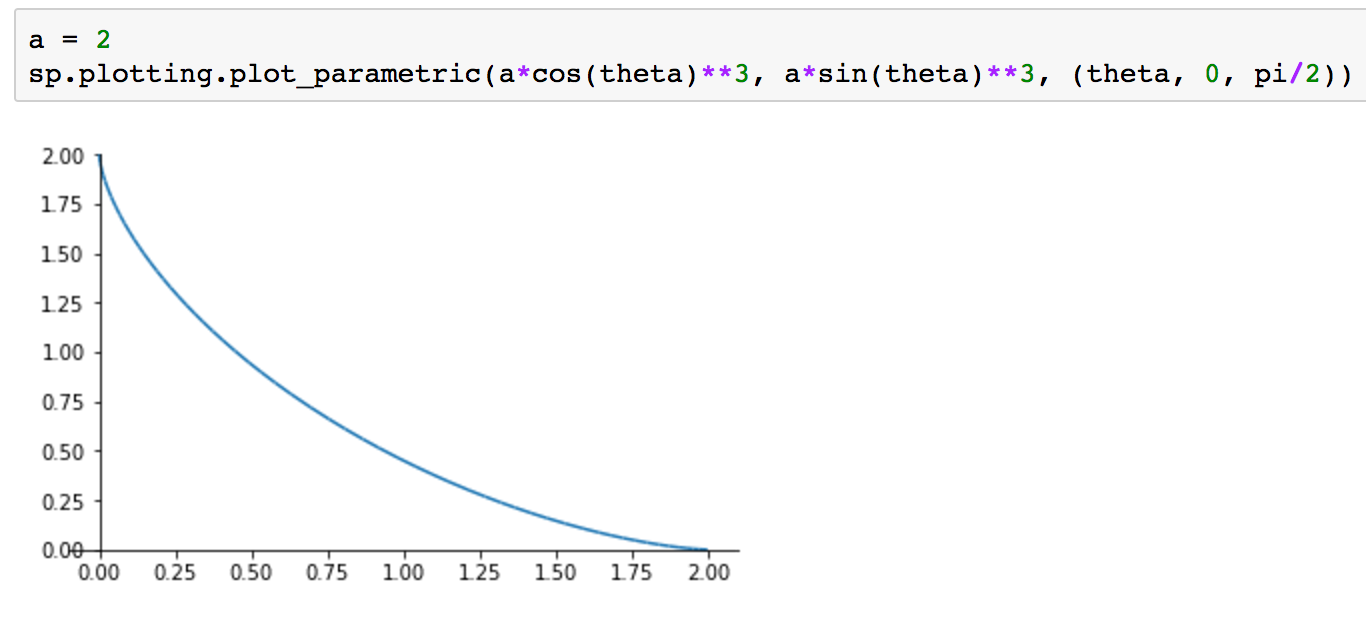
\includegraphics[width=500pt]{img/10-2-63.png}

\begin{mdframed}
  \begin{align*}
    A &= \int_0^{\pi/2} 2\pi y \sqrt{\dx^2 + \dy^2}\\
      &= \int_0^{\pi/2} 2\pi a\sin^3\theta \sqrt{(-3a\sin\theta\cos^2\theta)^2 +
                                                (3a\cos\theta\sin^2\theta)^2} \dtheta\\
      &= \int_0^{\pi/2} 2\pi a\sin^3\theta \sqrt{9a^2\sin^2\theta\cos^4\theta +
                                                9a^2\cos^2\theta\sin^4\theta} \dtheta\\
      &= \int_0^{\pi/2} 2\pi a\sin^3\theta 3a\sin\theta\cos\theta \sqrt{\cos^2 + \sin^2\theta} \dtheta\\
      &= 6\pi a^2\int_0^{\pi/2} \sin^4\theta \cos\theta \dtheta\\
      &= 6\pi a^2 \left[\frac{1}{5}\sin^5\theta \dtheta \right]_0^{\pi/2}\\
      &= \frac{6}{5}\pi a^2  ~~~ \checkmark
  \end{align*}
\end{mdframed}

\newpage
\subsection*{10.2.65}
Find the surface area generated by rotating the curve about the y-axis:
\begin{align*}
  x = 3t^2, ~~~ y = 2t^3, ~~~ 0 \leq t \leq 5
\end{align*}

\begin{mdframed}
  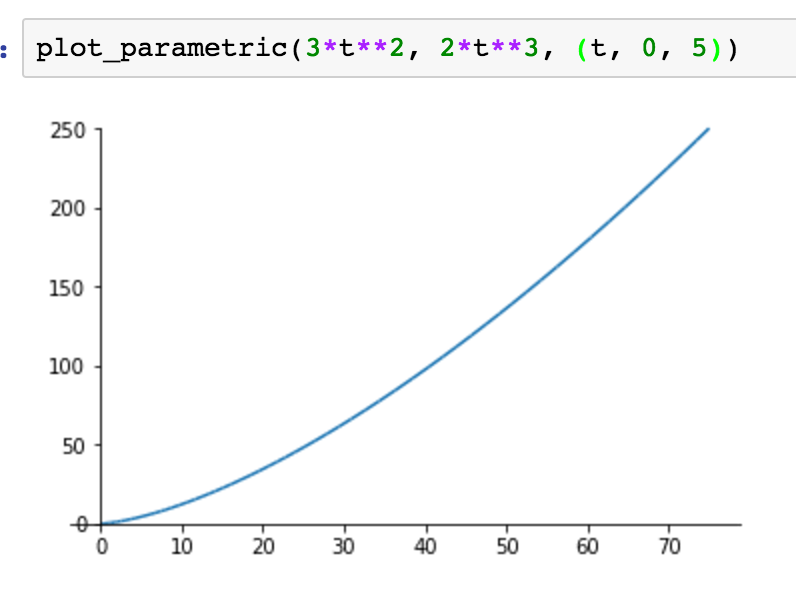
\includegraphics[width=400pt]{img/10-2-66.png}

  \begin{align*}
    A &= \int_{t=0}^{t=5} 2\pi x \sqrt{\dx^2 + \dy^2}\\
      &= \int_{t=0}^{t=5} 2\pi 3t^2 \sqrt{6^2t^2 + 6^2t^4} \dt\\
      &= 36\pi \int_{t=0}^{t=5} t^3 \sqrt{1 + t^2} \dt\\
  \end{align*}
  (Stewart answers really do seem to have a mistake this time?)
\end{mdframed}

\subsection*{10.2.65}
...

\subsection*{10.3.17}
Identify the curve by finding a Cartesian equation for the curve
\begin{align*}
  r = 5\cos\theta.
\end{align*}
\begin{mdframed}
  We want an expression involving $x$ and $y$: a condition that points $(x, y)$
  must satisfy in order to belong to the curve. We have
  \begin{align*}
    r &= 5\cos\theta\\
    r^2 &= 5r\cos\theta\\
    x^2 + y^2 &= 5x\\
    x^2 - 5x + y^2 &= 0\\
    \(x - \frac{5}{2}\)^2 + y^2 &= \frac{25}{4}\\
  \end{align*}
  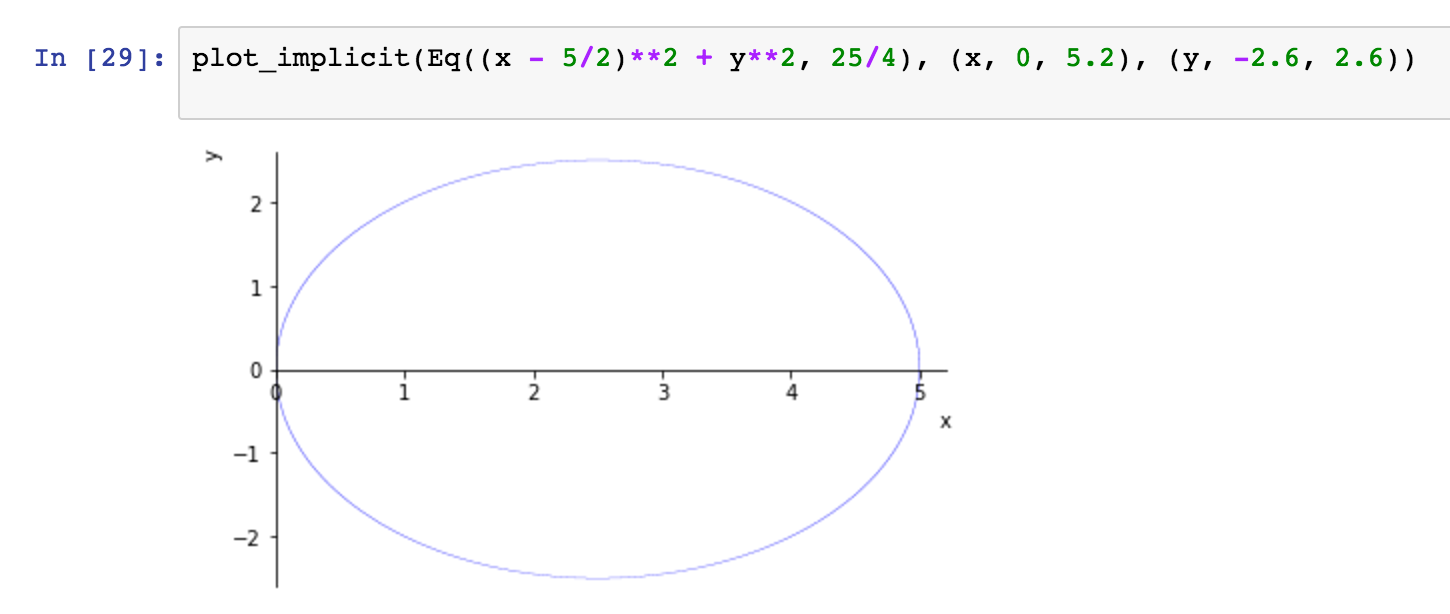
\includegraphics[width=300pt]{img/10-3-17-a.png}

  ~\\
  This isn't the requested answer, but if for some reason you wanted to
  parameterize the $x$ and $y$ coordinates as a function of $r$, then
  \begin{align*}
    x = r\cos\theta = \frac{r^2}{5},
  \end{align*}
  and
  \begin{align*}
    r^2 = 25(1 - \sin^2\theta)\\
    y = r\sin\theta = r\sqrt{1 - \frac{r^2}{25}}.
  \end{align*}
  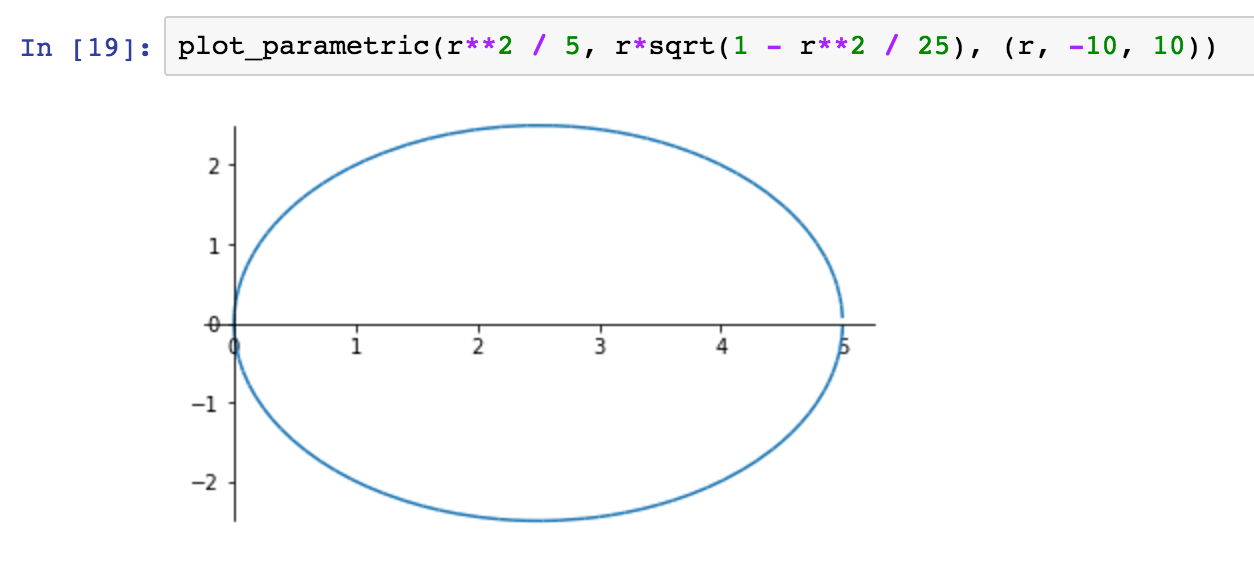
\includegraphics[width=300pt]{img/10-3-17.png}
\end{mdframed}

\subsection*{10.3.18}
Identify the curve by finding a Cartesian equation for the curve
\begin{align*}
  \theta = \pi/3.
\end{align*}

\begin{mdframed}
  \begin{align*}
    \sin\theta &= \frac{\sqrt{3}}{2}\\
    \cos\theta &= \frac{1}{2}\\
    \frac{y}{x} &= \frac{\sin\theta}{\cos\theta} = \sqrt{3}\\
    y &= \sqrt{3}x
  \end{align*}
\end{mdframed}

\subsection*{10.3.21}
Find a polar equation for the Cartesian equation $y = 2$.
\begin{mdframed}
  \begin{align*}
    r\sin\theta = 2
  \end{align*}
\end{mdframed}

\subsection*{10.3.22}
Find a polar equation for the Cartesian equation $y = x$.
\begin{mdframed}
  \begin{align*}
    \theta = \frac{\pi}{4}
  \end{align*}
\end{mdframed}

\subsection*{10.3.25}
Find a polar equation for the Cartesian equation $x^2 + y^2 = 2cx$.
\begin{mdframed}
  \begin{align*}
    r^2 \cos^2\theta + r^2\sin^2\theta &= 2cr\cos\theta\\
    r^2 &= 2cr\cos\theta\\
    r &= 2c\cos\theta
  \end{align*}
  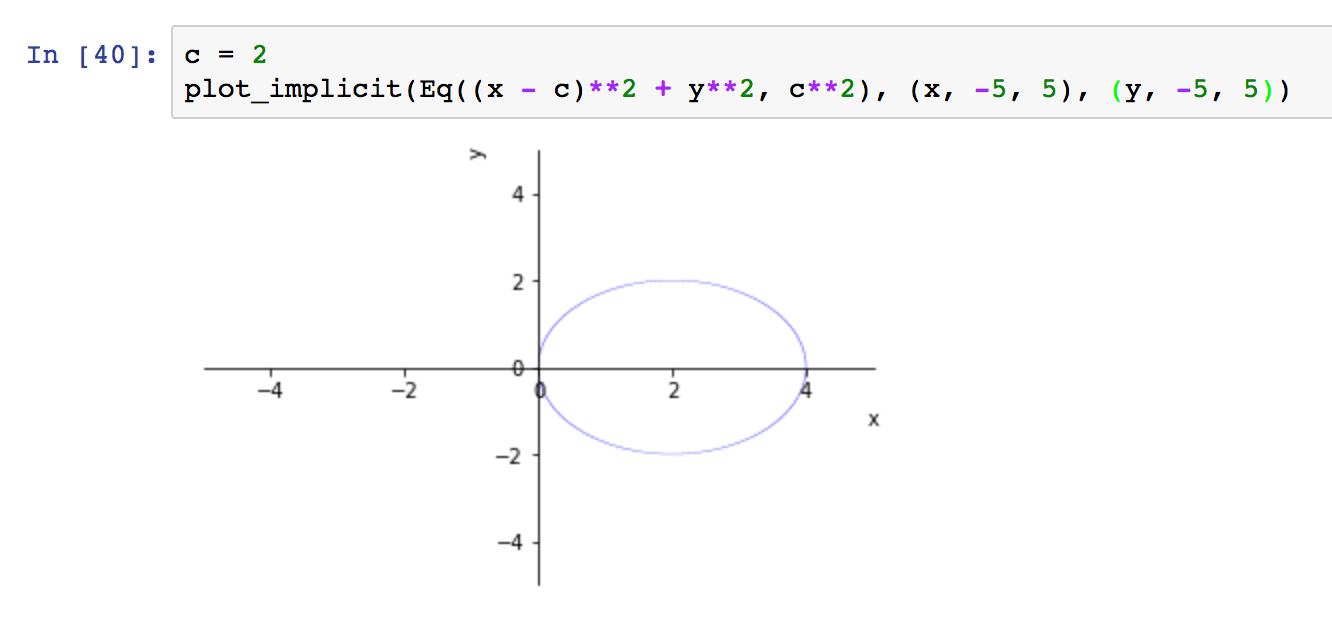
\includegraphics[width=300pt]{img/10-3-25-1.png}\\
  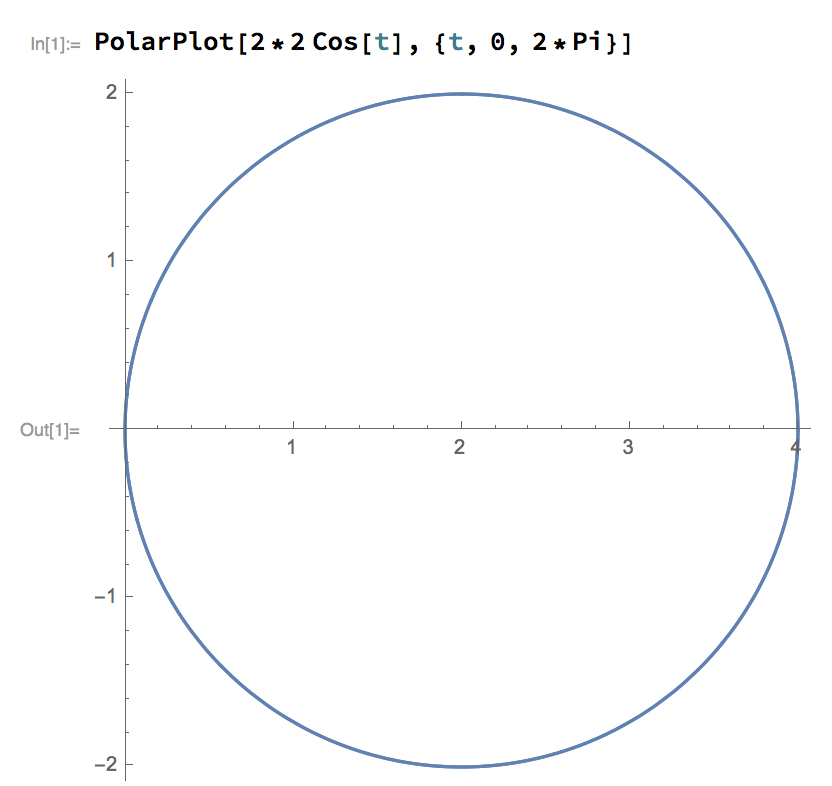
\includegraphics[width=200pt]{img/10-3-25-2.png}
\end{mdframed}

\newpage
\subsection*{10.3.29}
Sketch the curve in polar coordinates by first sketching $r$ as a function of
$\theta$ in Cartesian coordinates: $r = -2\sin\theta$.
\begin{mdframed}
  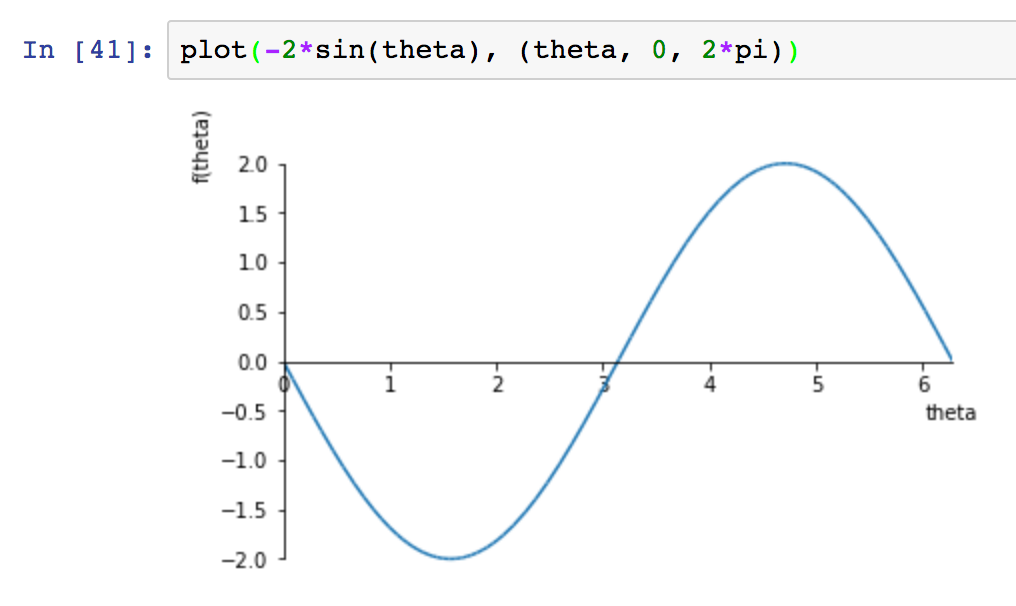
\includegraphics[width=300pt]{img/10-3-29-1.png}\\
  Now,
  \begin{align*}
    r &= -2\sin\theta\\
    r^2 &= -2r\sin\theta\\
    x^2 + y^2 &= -2y\\
    x^2 + (y+1)^2 &= 1,
  \end{align*}
  so it should be a circle with radius 1, shifted down 1 units. I believe that
  the circle is traced once for $0 \leq \theta < \pi$, and again for
  $\pi \leq \theta < 2\pi$.\\\\
  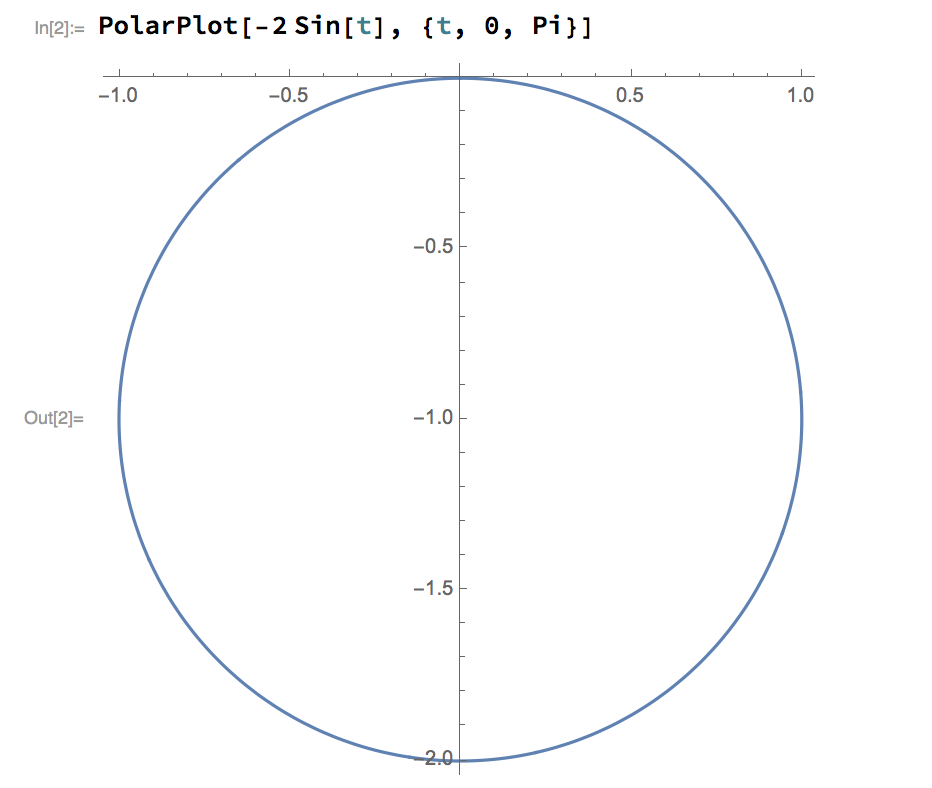
\includegraphics[width=200pt]{img/10-3-29-2.png}
  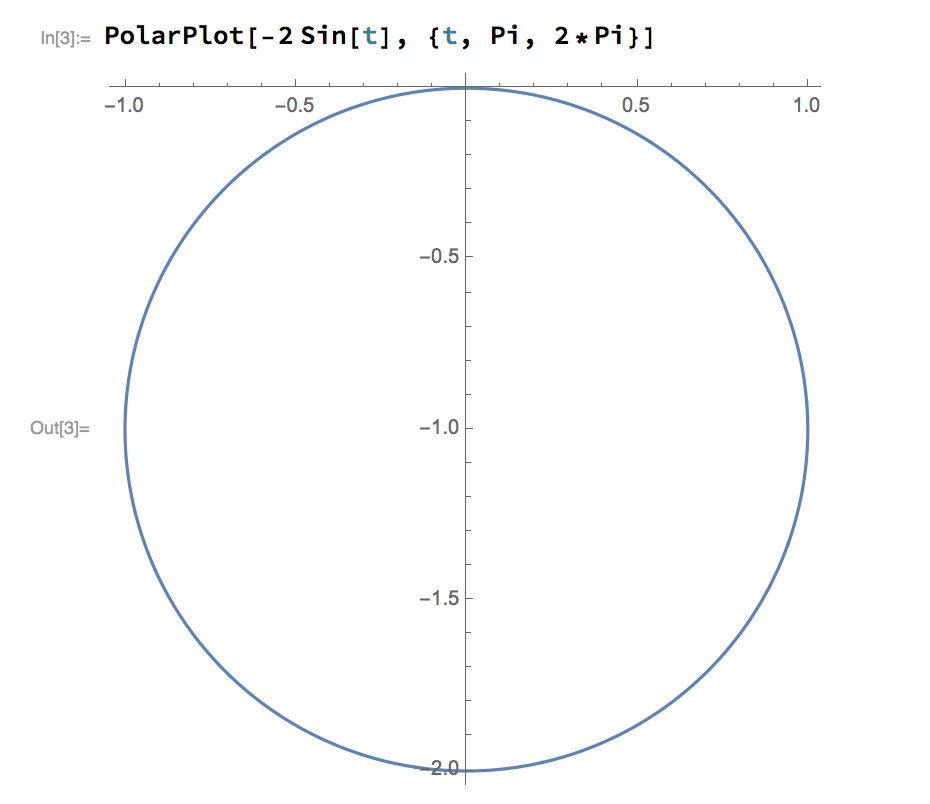
\includegraphics[width=200pt]{img/10-3-29-3.png}
  \\
\end{mdframed}

\newpage
\subsection*{10.3.30}
Sketch the curve in polar coordinates by first sketching $r$ as a function of
$\theta$ in Cartesian coordinates: $r = 1 - \cos\theta$.
\begin{mdframed}
  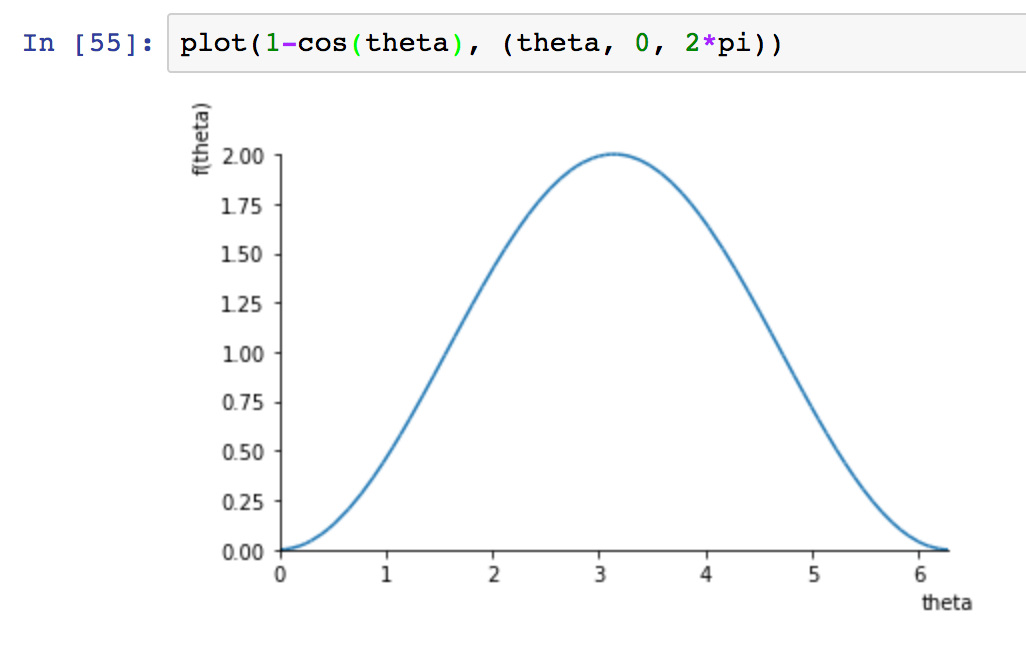
\includegraphics[width=300pt]{img/10-3-30.png}\\
  From which we can see that the graph is a cardioid.
  \begin{align*}
    r = 1 - \cos\theta\\
    r^2 = r - r\cos\theta\\
    x^2 + y^2 = \sqrt{x^2 + y^2} - x\\
    (x(x+1) + y^2)^2 = x^2 + y^2
  \end{align*}
  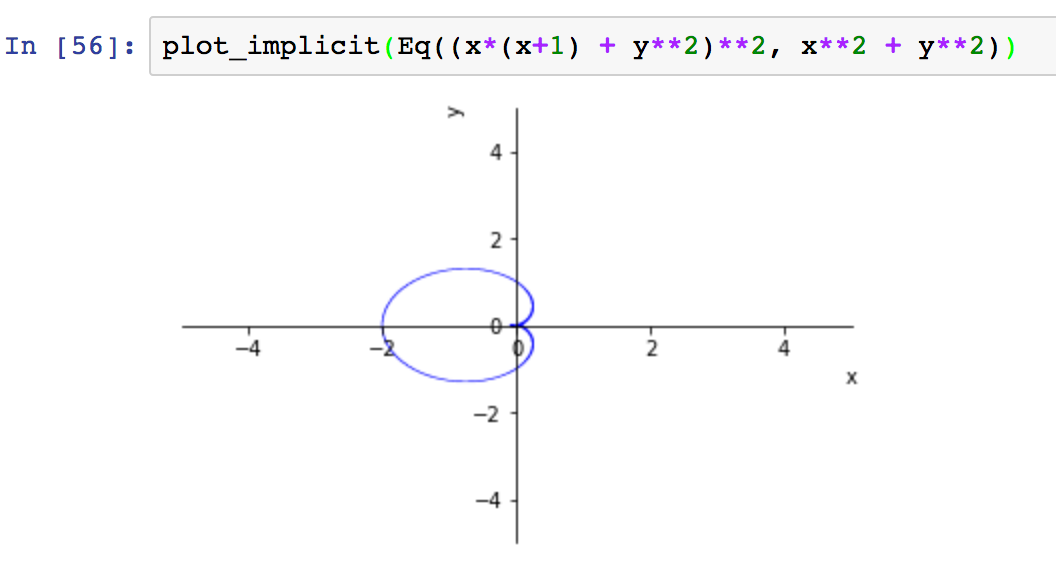
\includegraphics[width=400pt]{img/10-3-30-2.png}
\end{mdframed}

\subsection*{10.3.33}
Sketch the curve in polar coordinates by first sketching $r$ as a function of
$\theta$ in Cartesian coordinates: $r = \theta, \theta \geq 0$.
\begin{mdframed}
  It's a spiral.\\
  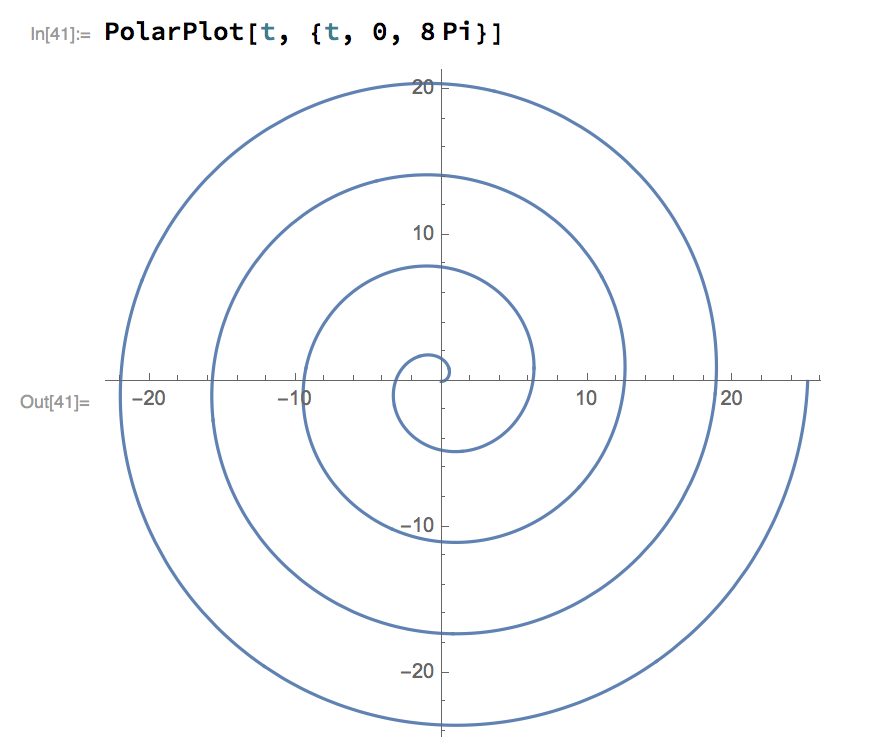
\includegraphics[width=300pt]{img/10-3-33.png}
\end{mdframed}

\newpage
\subsection*{10.3.35}
Sketch the curve in polar coordinates by first sketching $r$ as a function of
$\theta$ in Cartesian coordinates: $r = 3\cos(3\theta)$.
\begin{mdframed}
  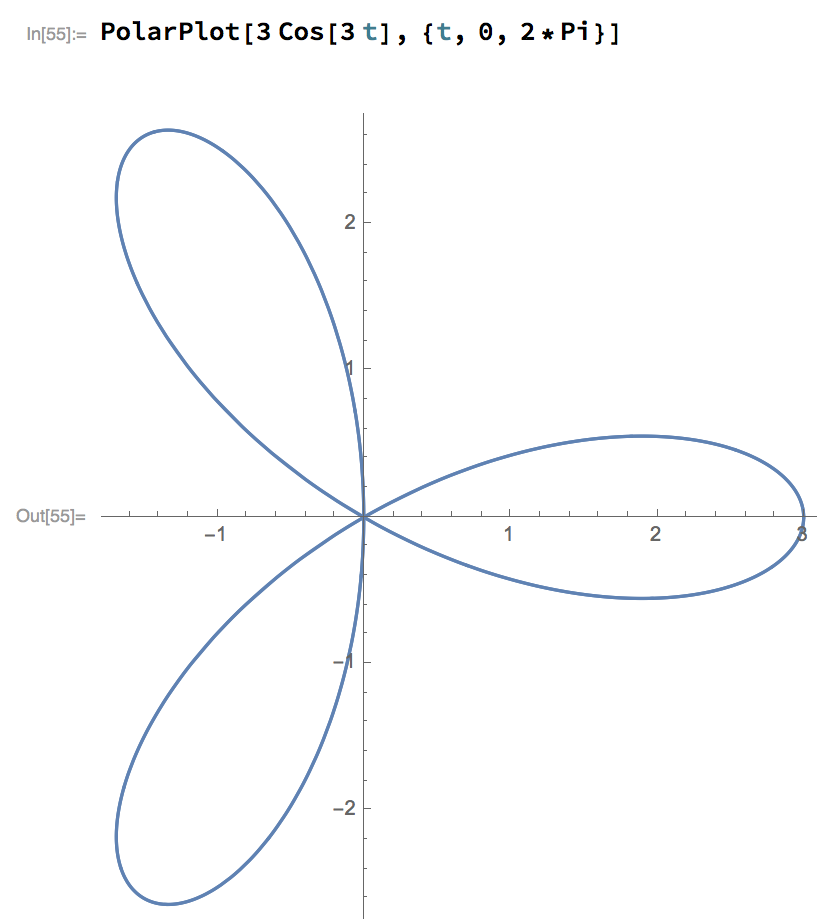
\includegraphics[width=300pt]{img/10-3-35.png}
\end{mdframed}

\newpage
\subsection*{10.3.56}
Find the slope of the tangent line to the polar curve, at $\theta$:\\
$r = 2 + \sin 3\theta, \theta=\pi/4$
\begin{mdframed}
  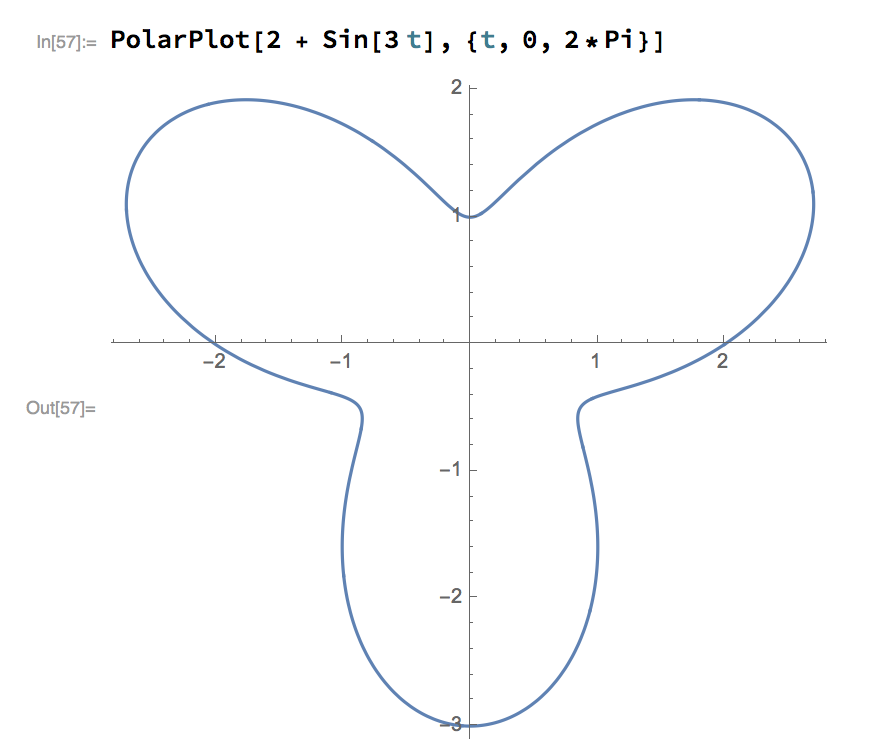
\includegraphics[width=200pt]{img/10-3-56.png}\\
  It looks like the slope might be -1. We use the chain rule, $\dydx = \(\dydtheta\)/\(\dxdtheta\)$ and so we need
  $\dxdtheta$ and $\dydtheta$.
\begin{align*}
  x          &= r\cos\theta = (2 + \sin 3\theta)\cos\theta\\
  \dxdtheta  &= (3\cos 3\theta)\cos\theta - (2 + \sin 3\theta)\sin\theta\\
  y          &= r\sin\theta = (2 + \sin 3\theta)\sin\theta\\
  \dydtheta  &= (3\cos 3\theta)\sin\theta + (2 + \sin 3\theta)\cos\theta\\
  \dydx &= \frac{\dydtheta}{\dxdtheta}\\
        &= \frac{(3\cos 3\theta)\sin\theta + (2 + \sin 3\theta)\cos\theta}
                {(3\cos 3\theta)\cos\theta - (2 + \sin 3\theta)\sin\theta}
\end{align*}
At $\theta=\pi/4$ this evaluates to
\begin{align*}
  \dydx
  &= \frac{\frac{-3}{\sqrt{2}}\frac{1}{\sqrt{2}} + (2 + \frac{1}{\sqrt{2}})\frac{1}{\sqrt{2}}}
          {\frac{-3}{\sqrt{2}}\frac{1}{\sqrt{2}} - (2 + \frac{1}{\sqrt{2}})\frac{1}{\sqrt{2}}}\\
  &= \frac{ 2\sqrt{2} - 2}
          {-2\sqrt{2} - 4}
  = \frac{ \sqrt{2} - 1}
         {-\sqrt{2} - 2} \approx -0.12 ~~~ \checkmark
\end{align*}
\end{mdframed}

\newpage
\subsection*{10.3.57}
Find the slope of the tangent line to the polar curve, at $\theta$:\\
$r = 1/\theta$, ~~~~~~$\theta = \pi$.
\begin{mdframed}
  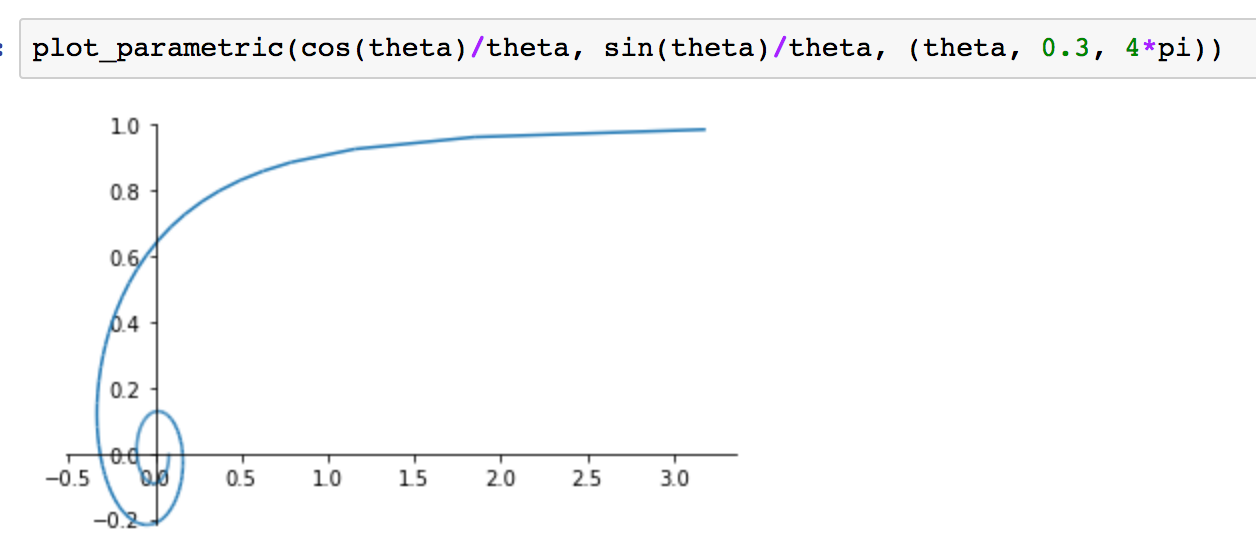
\includegraphics[width=300pt]{img/10-3-57.png}\\
  If I'm understanding this correctly, even as $\theta \to 0$, the
  y-coordinates aproaches 1 (since $\lim_{\theta \to 0}\frac{\sin\theta}{\theta} = 1$).

  Anyway, at $\theta=\pi$, the slope is negative something (hard to tell with sympy's aspect ratio).
  \begin{align*}
    \dydtheta
    &= \ddtheta \frac{\sin\theta}{\theta}
     = \frac{\theta \cos\theta - \sin\theta}{\theta^2}\\
    \\
    \dxdtheta
    &= \ddtheta \frac{\cos\theta}{\theta}
     = \frac{-\theta\sin\theta  - \cos\theta}{\theta^2}\\
    \\
    \dydx &= \frac{\theta \cos\theta - \sin\theta}
                  {-\theta\sin\theta  - \cos\theta}
  \end{align*}
  At $\theta=\pi$ this is $-\pi$. ~~~ \checkmark
\end{mdframed}

\newpage
\subsection*{10.3.61}
Find the points where the tangent is horizontal or vertical.
$r = 3\cos\theta$
\begin{mdframed}
  This is a circle with radius $3/2$, centered at $(3/2, 0)$. So the tangent is
  vertical at $\theta = k\frac{\pi}{2}$ for $k \in \Z$ (the left and right
  extrema of the circle). It's less clear where it is horizontal:
  \begin{align*}
    y &= \sin\theta\cos\theta\\
    \dydtheta &= \cos^2\theta -\sin^2\theta\\
    \\
    x &= \cos^2\theta\\
    \dxdtheta  &= -2\sin\theta\cos\theta\\
  \end{align*}
  As expected, $\dxdtheta = 0$ (tangent vertical) at
  $\theta = k\frac{\pi}{2}, k=0, 1, 2, ...$.\\
  And $\dydtheta = 0$ (tangent horizontal) at
  $\theta = k\frac{\pi}{4}, k=1,3,5,...$.
\end{mdframed}

\subsection*{10.3.63}
Find the points where the tangent is horizontal or vertical.
$r = 1 + \cos\theta$

\newpage
\subsection*{10.3.65}

Show that the polar equation $r = a\sin\theta + b\cos\theta$, where
$ab \neq 0$, represents a circle, and find its center and radius.\\
\begin{mdframed}
  The general Cartesian equation of a circle is
  \begin{align*}
    (x - c)^2 + (y - d)^2 = e^2,
  \end{align*}
  which is centered at $(c, d)$ with radius $e$. We have
  \begin{align*}
    r &= a\sin\theta + b\cos\theta\\
    r^2 &= ar\sin\theta + br\cos\theta\\
    x^2 + y^2 - ay - bx &= 0\\
    \(x - \frac{b}{2}\)^2 + \(y - \frac{a}{2}\)^2 &= \frac{a^2 + b^2}{4},
  \end{align*}
  so centered at $\(\frac{b}{2}, \frac{a}{2}\)$ with radius $\frac{\sqrt{a^2 + b^2}}{2}$. \checkmark
\end{mdframed}


\newpage
\subsection*{10.3.49}
Show that the polar curve $r = 4 + 2\sec\theta$ (a conchoid) has the line $x=2$
as a vertical asymptote by showing that $\lim_{r \to \pm \infty} x = 2$.\\
\begin{mdframed}
  \begin{align*}
    r &= 4 +\frac{2}{\cos\theta} \iff \cos\theta =\frac{2}{(r-4)}\\
    x &= r\cos\theta =\frac{2r}{(r-4)} = \frac{2}{1-4/r}\\
    \lim_{r \to \pm\infty} x &= 2
  \end{align*}
\end{mdframed}


\newpage
\subsection*{10.3.66}
Show that the curves $r = a\sin\theta$ and $r = a\cos\theta$ intersect at right
angles.
\begin{mdframed}
  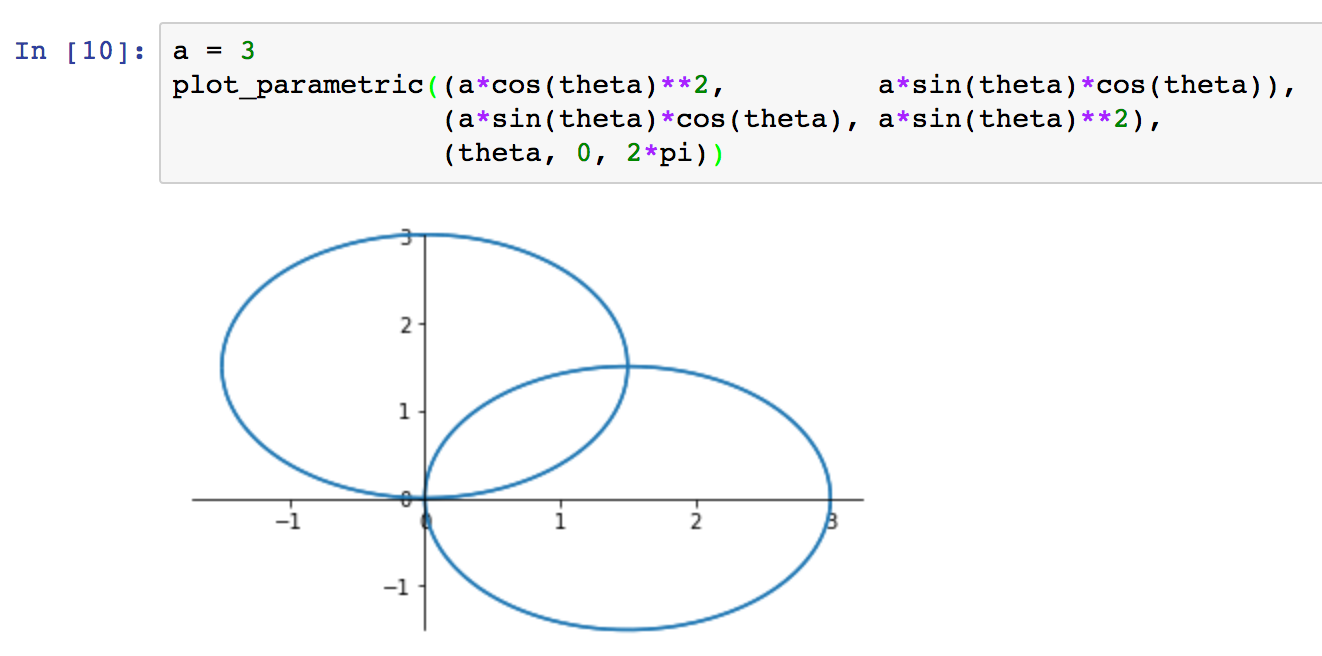
\includegraphics[width=300pt]{img/10-3-66.png}\\
  Strategy:
  \begin{enumerate}
  \item Determine intersection
  \item Determine tangents at intersection
  \item Show that these are orthogonal
  \end{enumerate}

  \subsubsection*{Cartesian coordinates}

  \textbf{Determine intersection}\\
  Multiplying the original polar equations on both sides by $r$, we see that in
  Cartesian coordinates, we require points $(x, y)$ that satisfy
  \begin{align*}
    \begin{cases}
      x^2 + y^2 &= ay\\
      x^2 + y^2 &= ax.
    \end{cases}
  \end{align*}
  Clearly the two equations together imply $y = x$, since $a > 0$. Substituting
  into the first equation, this gives
  \begin{align*}
    2y^2 &= ay \iff y(2y - a) = 0 \iff y = 0 \text{~~or~~} y = \frac{a}{2}.
  \end{align*}
  The first equation is equivalent to $x = \sqrt{ay - y^2}$, so the solutions
  are $(0, 0)$ and $(\frac{a}{2}, \frac{a}{2})$.

  \textbf{Determine tangents}\\
  For the first curve we have
  \begin{align*}
    x^2 + y^2 - ay = 0.
  \end{align*}
  Viewed as a function $\R^2 \to \R$, $\dx$ and $\dy$ must satisfy
  \begin{align*}
    2x \dx + (2y - a) \dy &= 0\\
    \implies \dydx &= \frac{-2x}{2y - a}.\\
                   &= 0, \infty \text{~~at~~} \(0, 0\), \(\frac{a}{2}, \frac{a}{2}\).
  \end{align*}

  Similarly for the other curve we have
  \begin{align*}
    x^2 + y^2 - ax &= 0\\
    (2x - a) \dx + 2y \dy &= 0\\
    \dydx &= \frac{a - 2x}{2y}\\
          &= \infty, 0  \text{~~at~~} \(0, 0\), \(\frac{a}{2}, \frac{a}{2}\).
  \end{align*}

  \textbf{Show that these are orthogonal}

  Show that the dot product is zero between vectors having the same direction
  as the tangents.

  That sounds sensible, but it is kind of clear from the values of $\dydx$
  above that they are orthogonal at both points of intersection.



  \newpage
  \subsubsection*{Polar coordinates}

  \textbf{Determine intersection}\\
  We need to find points $(r, \theta)$ that satisfy
  \begin{align*}
    \begin{cases}
      r &= a\sin\theta\\
      r &= a\cos\theta.
    \end{cases}
  \end{align*}
  Clearly such points lie on the diagonal $\tan\theta = 1$, i.e.
  $\theta = \frac{\pi}{4}$. Substituting into either equation gives
  $r = \frac{a}{\sqrt{2}}$, so one of the points of intersection is
  $\(\frac{a}{\sqrt{2}}, \frac{\pi}{4}\)$. The other one is at the origin but I
  seem to be struggling to make that come out of the algebra.

  \textbf{Determine tangents}\\
  We examine $\dydtheta$ and $\dxdtheta$.

  For the first curve
  \begin{align*}
    y         &= r\sin\theta = a\sin^2\theta\\
    \dydtheta &= 2a\sin\theta\cos\theta = a\sin 2\theta\\
              &= a \text{~~when~~} \theta=\frac{\pi}{4}\\
    \\
    x         &= r\cos\theta = a\sin\theta\cos\theta = \frac{a}{2}\sin 2 \theta\\
    \dxdtheta &= a\cos 2\theta\\
              &= 0 \text{~~when~~} \theta = \frac{\pi}{4},
  \end{align*}
  so the first curve has a vertical tangent at $\theta=\frac{\pi}{4}$.

  For the second curve
  \begin{align*}
    x         &= r\cos\theta = a\cos^2\theta\\
    \dxdtheta &= -2a\sin\theta\cos\theta = -a\sin 2\theta\\
              &= -a \text{~~when~~} \theta=\frac{\pi}{4}\\
    \\
    y         &= r\sin\theta = a\sin\theta\cos\theta = \frac{a}{2}\sin 2 \theta\\
    \dydtheta &= a\cos 2\theta\\
              &= 0 \text{~~when~~} \theta = \frac{\pi}{4}.
  \end{align*}
  so the second curve has a horizontal tangent at $\theta=\frac{\pi}{4}$.

  Therefore the two curves intersect at right-angles when $\theta=\frac{\pi}{4}$.


\end{mdframed}


\newpage
\subsection*{10.4.2}
Find the area of the region
\begin{align*}
  r = \cos\theta, ~~~ 0 \leq \theta \leq \pi/6
\end{align*}
\begin{mdframed}
  The curve describes a circle. Note that a sector subtended by $2\pi$ radians
  has area $\pi r^2$, therefore a sector of $\d\theta$ radians has area
  $\frac{\d\theta}{2}r^2$. The requested area is
\begin{align*}
  \int_0^{\pi/6} \frac{\d\theta}{2}r^2
  &= \int_0^{\pi/6} \frac{\d\theta}{2}\cos^2\theta.\\
\end{align*}
Let $I = \int \cos^2\theta \dtheta$. Integration by parts
\begin{align*}
  \d(u v) &= u\d v + v\du\\
   uv &= \int u \d v + \int v \du\\
  \int u \d v &= uv - \int v \du
\end{align*}
gives
\begin{align*}
  u &= \cos\theta\\
  \d v  &= \cos\theta \dtheta\\
  I = \int \cos^2 \theta \d\theta &= \cos\theta\sin\theta + \int \sin^2\theta \dtheta\\
    &= \cos\theta\sin\theta + \theta - I\\
    &= \frac{1}{2}\(\cos\theta\sin\theta + \theta\) + C\\
    &= \frac{1}{4}\sin 2\theta + \frac{\theta}{2} + C
\end{align*}
Thus the requested area is
\begin{align*}
  \frac{1}{8} \sin 2\theta + \frac{1}{4}\theta \Big|^{\pi/6}_0
  &= \frac{1}{8}\sin\frac{\pi}{3} + \frac{\pi}{24} = \frac{\sqrt{3}}{16} + \frac{\pi}{24}. \checkmark
\end{align*}
\end{mdframed}

\subsection*{10.4.5}
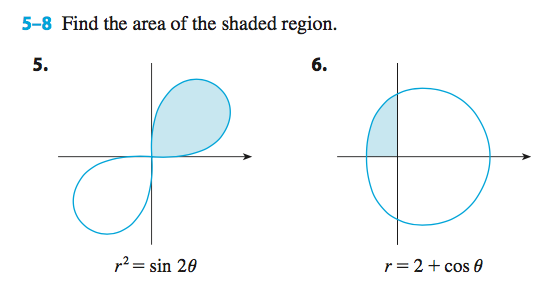
\includegraphics[width=200pt]{img/10-4-5-6.png}
\begin{mdframed}
  Note that a sector subtended by $\theta$ radians has area
  $\pi r^2 \cdot \frac{\theta}{2\pi} = \frac{\theta}{2}r^2$.\\\\
  \textbf{5.} The area is
  \begin{align*}
    \int_0^{\pi/2} \frac{\d\theta}{2}\sin2\theta = -\frac{1}{4}\cos2\theta\Big|_0^{\pi/2} = -\frac{1}{4}(-1 - 1) = \frac{1}{2}.
  \end{align*}\\
  \textbf{6.} The area is
  \begin{align*}
    \int_{\pi/2}^\pi \frac{1}{2}\big(2 + \cos\theta\big)^2 \d\theta\\
  \end{align*}
\end{mdframed}

\subsection*{10.4.6}
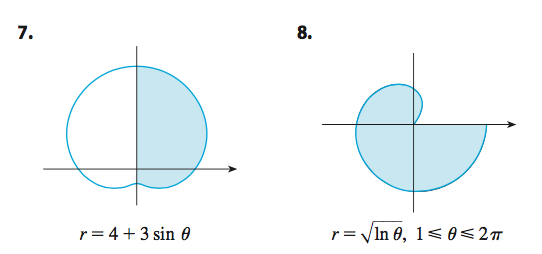
\includegraphics[width=300pt]{img/10-4-7-8.png}
\begin{mdframed}
  \textbf{7.} The area is $\int_{-3\pi/2}^{\pi/2}\frac{\d\theta}{2}(4 + 3\sin\theta)^2$
\end{mdframed}

\subsection*{10.4.7}
\subsection*{10.4.9}
\subsection*{10.4.10}
\subsection*{10.4.17}
\subsection*{10.4.18}
\subsection*{10.4.23}
\subsection*{10.4.24}
\subsection*{10.4.27}
\subsection*{10.4.28}
\subsection*{10.4.29}
\subsection*{10.4.30}
\subsection*{10.4.31}
\subsection*{10.4.32}
\subsection*{10.4.37}
\subsection*{10.4.38}
\subsection*{10.4.39}
\subsection*{10.4.41}
\subsection*{10.4.45}
\subsection*{10.4.47}
\subsection*{10.4.55}

\subsection*{12.1.3}
\subsection*{12.1.6}
\subsection*{12.1.7}
\subsection*{12.1.9}
\subsection*{12.1.11}
\subsection*{12.1.17}
\subsection*{12.1.25}
\subsection*{12.1.27}
\subsection*{12.1.30}
\subsection*{12.1.31}
\subsection*{12.1.32}
\subsection*{12.1.35}
\subsection*{12.1.39}
\subsection*{12.1.40}
\subsection*{12.1.41}
\subsection*{12.1.44}


\subsection{Example 7: The Cycloid}
The curve traced out by a point $P$ on the circumference of a circle as the
circle rolls along a straight line is called a cycloid. If the circle has
radius $r$ and rolls along the $x$-axis and if one position of $P$ is the
origin, find parametric equations for the cycloid.
\begin{mdframed}
  ...
\end{mdframed}
\section{Math 53 Midterm I Februrary 2011 Frenkel}

1. Consider the curve in $\R^2$ defined by the equation

$$
r = \cos(2\theta)
$$.

(a) Sketch this curve.

(b) Find the area of the region enclosed by one loop of this curve.\\

\begin{mdframed}
  The area of a sector of $\dtheta$ radians is $\frac{\dtheta}{2\pi}\pi r^2 = \frac{\dtheta}{2}\cos^2(2\theta)$. Recall the identity $\cos^2 t = \frac{1}{2} + \frac{1}{2}\cos(2t)$. Therefore the area of one loop is

\begin{align*}
  \int_{-\pi/4}^{\pi/4} \frac{\dtheta}{2}\cos^2(2\theta)
  =&\frac{1}{4}\int_{-\pi/4}^{\pi/4} (1 + \cos 4\theta) \dtheta \\
  =& \Big|\frac{1}{4} + \frac{1}{16}\sin(4\theta)\Big|_{-\pi/4}^{\pi/4} \\
  =& \frac{\pi}{8}.
\end{align*}

\end{mdframed}~\\

2. Find an equation of the surface consisting of all points in $\R^3$ that are equidistant
from the point $(0, 0, 1)$ and the plane $z = 2$.\\

\begin{mdframed}
  Such points satisfy $\sqrt{x^2 + y^2 + (z - 1)^2} = z - 2$, which simplifies as

\begin{align*}
x^2 + y^2 + z^2 - 2z + 1 &= z^2 - 4z + 4 \\
z &= -\frac{x^2}{2} -\frac{y^2}{2} + \frac{3}{2} \\
\end{align*}

\end{mdframed}~\\

(b) Sketch this surface. What is it called?

\begin{mdframed}
  Concave-down paraboloid
\end{mdframed}

3. Show that the function $\frac{x^{50}y^{50}}{x^{100} + y^{200}}$ does not
have a limit at $(x, y) = (0, 0)$.

\begin{mdframed}
  First consider approaching $(0, 0)$ along the line $x=0$: this gives a limiting value of 0.
  Now consider approaching along the line $x=y$: this gives a limiting value of $\frac{x^{100}}{x^{100} + x^{200}} \to 1$.
  Since the two approaches gives different results, the limit does not exist.
\end{mdframed}~\\

4. Consider the function $f(x,y) = x\cos(y) + y^2e^x + x$.

(a) Find the differential of this function

\begin{mdframed}
  \begin{align*}
  \d f(x, y) &= \partiald{f}{x}\d x + \partiald{f}{y}\d y\\
             &= (\cos(y) + y^2e^x + 1)\d x + (-x\sin(y) + 2ye^x) \d y
  \end{align*}
\end{mdframed}

(b) Find an equation of the tangent plane to the graph of this function at the
point $(0, \pi, \pi^2)$.

\begin{mdframed}
  Points in the plane passing through $(x_0, y_0, z_0)$ satisfy
  \begin{align*}
    z - z_0 = (x - x_0)\partiald{f}{x} + (y - y_0)\partiald{f}{y},
  \end{align*}
  so in this case
  \begin{align*}
    z - \pi^2 &= (x - 0)\(\cos(\pi) + \pi^2e^0 + 1\) + (y - \pi)\(-0\sin(\pi) + 2\pi e^0\)\\
    z &= \pi^2x + 2\pi y - \pi^2
  \end{align*}
\end{mdframed}~\\

5. Suppose we need to know an equation of the tangent plane to a surface $S$ at
the point $P = (1, 3, 2)$. We don't have an equation for $S$, but we know that the
curves

\begin{align*}
r_1(t) &= \langle 1 + 5t,    3 - t^2,       2 + t - t^3    \rangle, \\
r_2(s) &= \langle 3s - 2s^2, s + s^3 + s^4, s - s^2 + 2s^3 \rangle
\end{align*}
both lie in $S$. Find an equation of the tangent plane to $S$ at the point $P$.


~\\\begin{mdframed}
  First note that $P$ lies in both curves, since $r_1(0) = r_2(1) = P$.

  Now we use the two curves to obtain two vectors that lie in the tangent
  plane. Their cross product is a vector normal to the tangent plane and provides
  the coefficients for the equation of the plane.

  The derivative of a curve $r(t)$ with respect to the parameter $t$ is a
  function giving a tangent vector. The derivatives are:

\begin{align*}
  \dot r_1(t) = \cveccc{5}{-2t}{1 - 3t^2}, ~~~
  \dot r_2(s) = \cveccc{3 - 4s}{1 + 3s^2 + 4s^3}{1 - 2s + 6s^2}.
\end{align*}

Evaluated at $P = \cveccc{1}{3}{2}$ these are

\begin{align*}
  \dot r_1(t) = \cveccc{5}{0}{1}, ~~~
  \dot r_2(s) = \cveccc{-1}{8}{5}.
\end{align*}

Their cross product is

\begin{align*}
  \cveccc{5}{0}{1} \times \cveccc{-1}{8}{5} =
  \cveccc{(0 \times 5) - (1 \times 8)}
         {(1 \times -1) - (5 \times 5)}
         {(5 \times 8) - (0 \times -1)} =
  \cveccc{-8}{-26}{40}
\end{align*}


Therefore points in the plane satisfy

\begin{align*}
  -8(x - x_0) - 26(y - y_0) + 40(z - z_0) = 0 \\
  -8(x - 1)   - 26(y - 3)   + 40(z - 2) = 0.
\end{align*}

Would another way of doing this, without using the cross product, be to start
by saying that the plane is the set of points $(x, y, z)$ that satisfy

\begin{align*}
  \cveccc{x}{y}{z} = \cveccc{1}{3}{2} + u\cveccc{5}{0}{1} + v \cveccc{-1}{8}{5},
\end{align*}

and then to somehow change basis/variables from $(u, v)$ to $(x, y)$?

\end{mdframed}


\end{document}